\documentclass[11pt]{article}
\usepackage{geometry, titlesec}
\usepackage[parfill]{parskip}
\usepackage[italicdiff]{physics}
\usepackage{amsfonts, amsthm}
\usepackage[cm]{fullpage}
\usepackage{fancyhdr}
\usepackage{enumitem}
\usepackage{xcolor, soul}
\usepackage{graphicx}
\usepackage[export]{adjustbox}
\usepackage{siunitx}
%\allowdisplaybreaks

\renewcommand{\thesubsection}{\thesection.\alph{subsection}}
\setenumerate[1]{label={(\alph*)}}

\makeatletter
\renewcommand*\env@cases[1][1.2]{%
  \let\@ifnextchar\new@ifnextchar
  \left\lbrace
  \def\arraystretch{#1}%
  \array{@{}l@{\quad}l@{}}%
}
\makeatother
 
\renewcommand{\footrulewidth}{.2pt}
%\setlist[enumerate]{leftmargin=*}
\pagestyle{fancy}
\fancyhf{}
\lhead{Physics 132-B}
\chead{\textbf{Discussion 7 Problems}}
\rhead{A--De Discussion}
\setlength{\headheight}{11pt}
\setlength{\headsep}{11pt}
\setlength{\footskip}{24pt}
\lfoot{\today}
\rfoot{\thepage}

\titleformat{\subsection}[runin]{\normalfont\large\bfseries}{\thesubsection}{1em}{}
\newcommand{\refeq}[1]{(\ref{#1})}

\newcommand{\beq}{\begin{equation*}}
\newcommand{\eeq}{\end{equation*}}

\newcommand{\beqn}{\begin{equation}}
\newcommand{\eeqn}{\end{equation}}

\newcommand{\blg}{\begin{align*}}
\newcommand{\elg}{\end{align*}}


\newenvironment{statement}
{
%    \color{gray}
    \ignorespaces
}
{
%    \smallskip
}

\newenvironment{problem}
{
%    \color{darkgray}
    \ignorespaces
}

\newenvironment{solution}
{
    \paragraph{Solution.}
    \ignorespaces
}
{
    \bigskip
}

\renewcommand{\vec}[1]{\mathbf{#1}}


\begin{document}
	


\newcommand{\vF}{\vb{F}}
\newcommand{\vv}{\vb{v}}
\newcommand{\vB}{\vb{B}}

\paragraph{Question 27.1}
\begin{problem}
	Can a charged particle move through a magnetic field without experiencing any force?  If so, how?  If not, why not?
\end{problem}

\begin{solution}
	The magnetic force on a particle of charge $q$ is given by $\vF = q \vv \times \vB$, where $\vv$ is the particle's velocity and $\vB$ is the magnetic field.  The cross product $\vv \times \vB$ is zero if $\vv$ and $\vB$ are parallel.  In this case, $\vF = 0$.  So yes, a charged particle can move through a magnetic field without experiencing any force, as long as it is moving parallel to the field.
\end{solution}

\vfill

\paragraph{Question 27.7}
\begin{problem}
	If the magnetic force does not work on a charged particle, how can it have any effect on the particle's motion?  Are there other examples of forces that do no work but have a significant effect on a particle's motion?
\end{problem}

\begin{solution}
	It is certainly possible for a force to affect motion without doing work.  Think back to the mechanics problems we studied last quarter, and imagine a hockey puck sliding horizontally on some (frictionless) ice.  If someone hits the puck (laterally) with a hockey stick, they are exerting a force on the puck, whose direction of motion will change depending on the direction of the force.  However, the potential energy of the puck hasn't changed, because it hasn't moved vertically.  The magnetic force similarly is able to change the direction of a particle without doing work.
\end{solution}

\vfill

\paragraph{Question 28.4}
\begin{problem}
	Two parallel conductors carrying current in the same direction attract each other.  If they are permitted to move toward each other, the forces of attraction do work.  From where does the energy come?  Does this contradict the assertion in Chapter 27 that magnetic forces on moving charges do no work?  Explain.
\end{problem}

\begin{solution}
	Magnetic forces are not the only thing we have to think about for this system.  The conductors are carrying current, so they must be connected to a power source.  The power source creates a potential difference which causes a current to flow.  The energy to do work on objects in the magnetic field between the conductors therefore comes from the power source.  This does not contradict the assumption that magnetic forces do no work.  The power source does the work; the magnetic field just delivers the force.
\end{solution}

\vfill
%\clearpage

\paragraph{Question 28.10}
\begin{problem}
	What are the relative advantages and disadvantages of Ampere's law and the law of Biot and Savart for practical calculations of magnetic fields?
\end{problem}

\begin{solution}
	This is like comparing Coulomb's law and Gauss's law.  Coulomb's law can tell us the electric field for \emph{any} charge distribution, but actually executing it usually involves calculus and can be difficult.  On the other hand, Gauss's law can only be used when we have certain symmetries, but it makes calculating the electric field in these cases very easy.
	
	Likewise, the Biot-Savart law can be used to calculate the magnetic field for \emph{any} current distribution, but it involes calculus and cross products.  Ampere's law can only be used for certain symmetric configurations, but it is mathematically much easier to implement when it is an option.
\end{solution}

\clearpage

%\begin{minipage}[l]{0.7\textwidth}
%\paragraph{Question 26.9}
%\begin{problem}
%	A light bulb is connected in the circuit shown in \textbf{Fig.~Q26.9}.  If we close the switch $S$, does the bulb's brightness increase, decrease, or stay the same?  Why?
%\end{problem}
%\end{minipage}%
%\hspace{0.05\textwidth}%
%\begin{minipage}{0.25\textwidth}
%\center 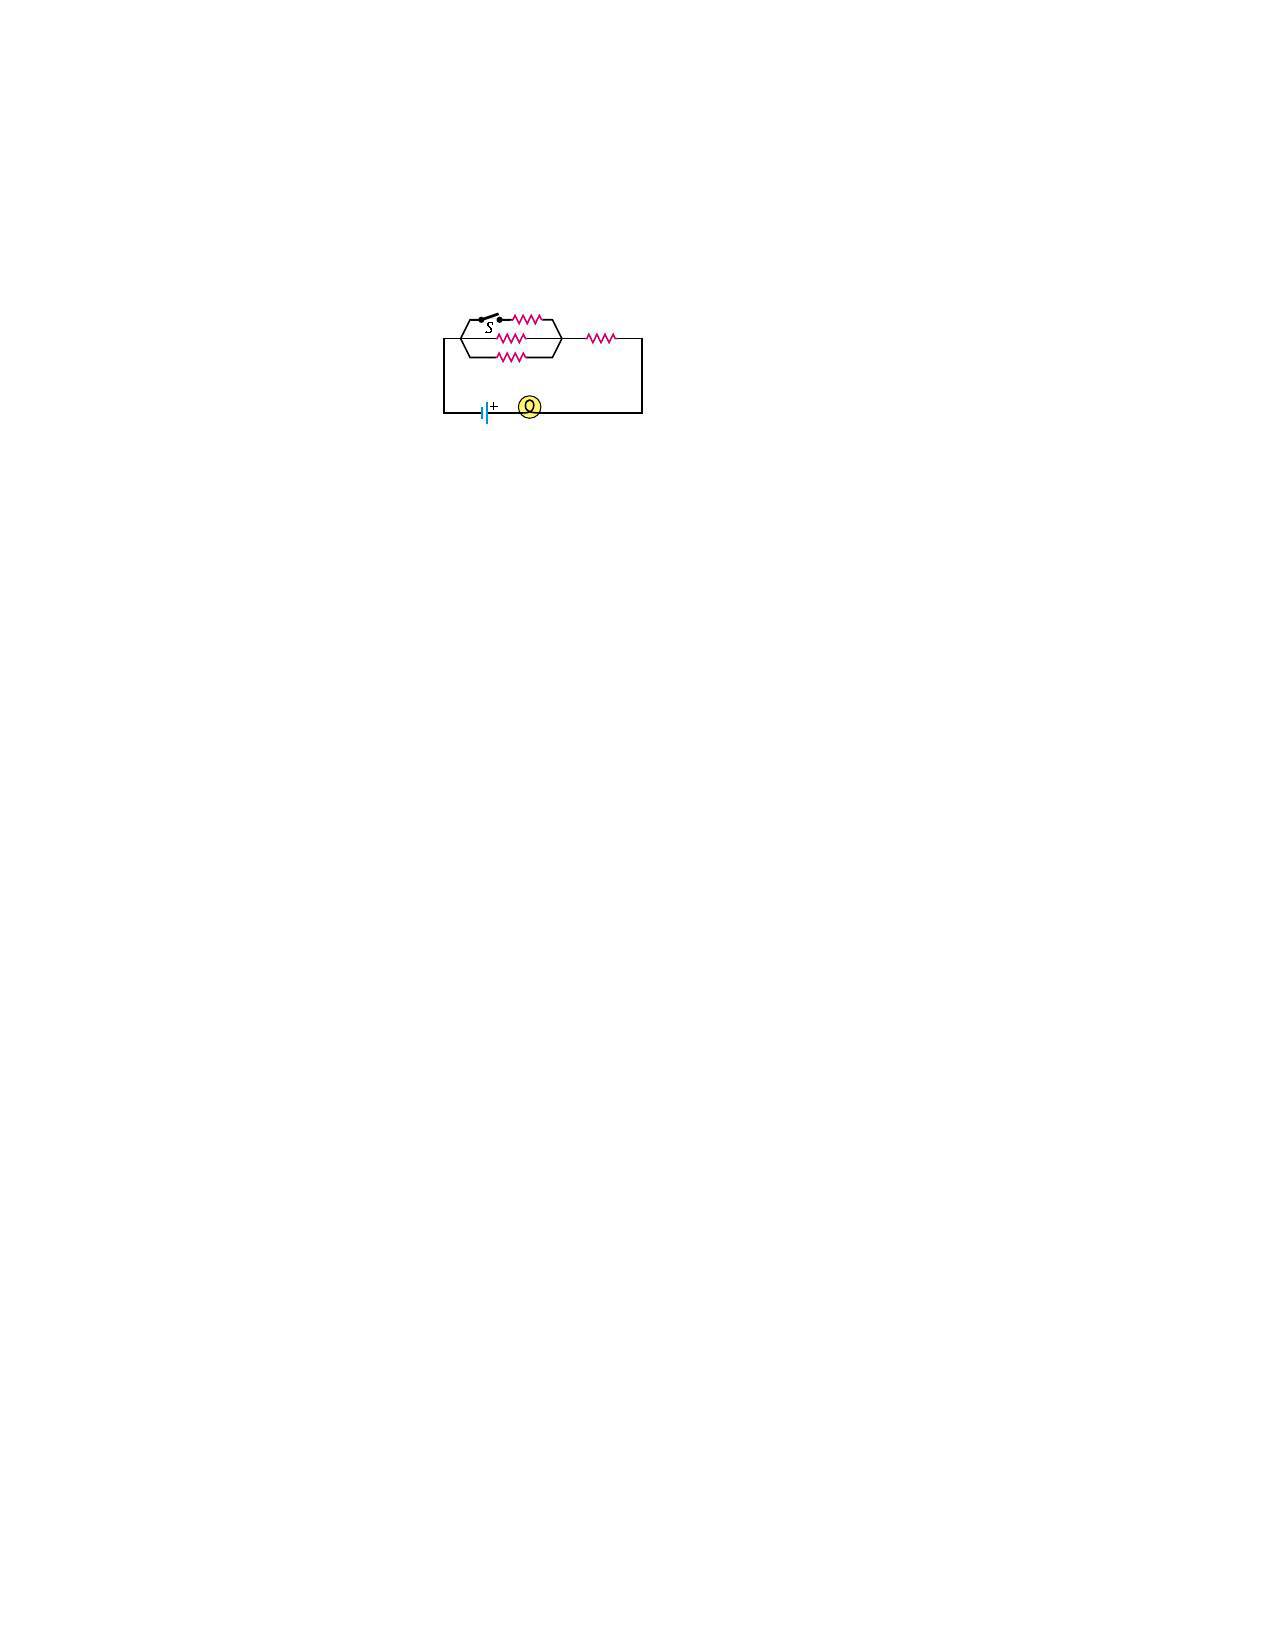
\includegraphics{Q26-9}
%\center \textbf{Figure Q26.9}
%\end{minipage}

\vfill 

\end{document}